General process

- divide the dataset in train and test
Learning the parameters of a prediction function and testing it on the same data is a methodological mistake: a model that would just repeat the labels of the samples that it has just seen would have a perfect score but would fail to predict anything useful on yet-unseen data. This situation is called overfitting. To avoid it, it is common practice when performing a (supervised) machine learning experiment to hold out part of the available data as a test set.
- learn and evaluate
- feature description
- choose of the classifier

presenting different channel representation
RGB, gray, HSV

\section{Feature descriptors}

\subsection{Local binary pattern}

% http://www.pyimagesearch.com/2015/12/07/local-binary-patterns-with-python-opencv/

Local binary pattern is a visual descriptor for texture composition of an image, first presented in 2002 in \cite{Ojala2002} (although the concept of LBPs were introduced as early as 1993).

The figure \ref{fig:lbp_process} represents an example of the LBP in which the LBP code of the center pixel (in red color and value 20) is used as a local intensity threshold : the neighbour pixels whose intensities are equal or higher than the center pixel’s are labeled as ”1”; otherwise as ”0”. Then, starting always from the same point, we can transform this binary string to decimal. In this example we start at the top-right point and work our way clockwise accumulating the binary string as we go along and obtain the value 24.

\begin{figure}[h]
    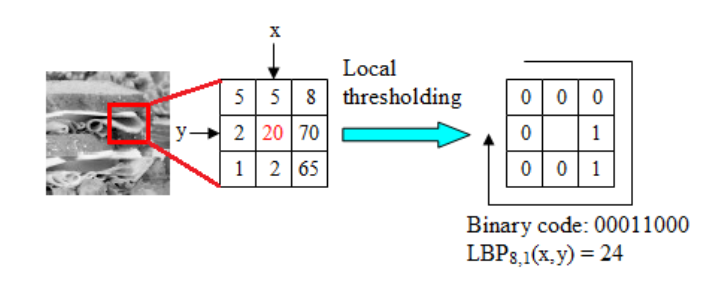
\includegraphics[scale=0.55]{img/lbp}
    \caption{Illustration of the LBP descriptor's process}
    \label{fig:lbp_process}
\end{figure}

We adopt the following notation. Given a pixel $c = (x_c, y_c)$, the value of the $LBP$ code of $c$ is defined as:
$$LBP_{P, R} (x_c, y_c) = \sum_{p = 0}^{P - 1} s (g_p - g_c) 2^p$$
where:
\begin{itemize}
    \item $p$ is a neighbour pixel of $c$ and the distance from $p$ to $c$ does not exceed $R$. thus, $R$ is the radius of a circle centered in $c$ and $P$ is the numbered of sampled points.
    \item $g_p$ and $g_c$ are the gray values (intensities) of $p$ and $c$
    \item $s(x)$ is the function defined as:
    \begin{equation}
    s(x) =
    \begin{cases}
    1 & \text{if $x \geq 0$}\\
    0 & \text{otherwise} \\
    \end{cases}
    \end{equation}
\end{itemize}

In Fig. \ref{fig:lbp_process}, $R$ and $P$ are 1 and 8 respectively.

The number of histograms bins for $LBP_{P, R}$ is $2^P$.

Lastly, it’s important that we consider the concept of LBP uniformity. A LBP is considered to be uniform if it has at most two 0-1 or 1-0 transitions. For example, the pattern 00001000  (2 transitions) and 10000000  (1 transition) are both considered to be uniform patterns since they contain at most two 0-1 and 1-0 transitions. The pattern 01010010 ) on the other hand is not considered a uniform pattern since it has six 0-1 or 1-0 transitions.

The number of uniform prototypes in a Local Binary Pattern is completely dependent on the number of points p. As the value of p increases, so will the dimensionality of your resulting histogram. Please refer to the original Ojala et al. paper for the full explanation on deriving the number of patterns and uniform patterns based on this value. However, for the time being simply keep in mind that given the number of points p in the LBP there are p + 1 uniform patterns. The final dimensionality of the histogram is thus p + 2, where the added entry tabulates all patterns that are not uniform.

\subsection{Color histogram}

HSV channels: Hue, Saturation and Value.
It has been defined to be closer to the way human represents colours.
Hue and Saturation corresponds to the chromaticity of the colour, Value to the lightness.
As value is really dependant of the condition where the picture were taken, we don't use it for color histogram.

\subsubsection{Color moments}

\subsection{The first two moments}

For a discrete random variable $X$, the first two moments are defined as:
\begin{itemize}
    \item \textbf{Expected value}: $$\E \left[ X \right] = \mu = \sum_{i = 1}^{n} p_i x_i $$
    \item \textbf{Variance}:  $$ \Var (X)= \E \left[ (X - \E \left[ X \right] )^2 \right] =\sum _{i=1}^{n} p_i (x_{i} - \mu )^{2} $$
\end{itemize}

\subsection{Hu moments}

\subsubsection{Raw moments}

For a two-dimensional continuous function f(x,y) the moment (sometimes called \enquote{raw moment}) of (p + q)th order is defined as: 
$$M_{pq}=\int \limits _{-\infty }^{\infty }\int \limits _{-\infty }^{\infty }x^{p}y^{q}f(x,y) dx dy $$
for $p$ and $q \in \N $

\subsubsection{Central moments}

And the central moments are :
$$\mu_{pq}=\int \limits_{-\infty }^{\infty }\int \limits _{-\infty}^{\infty} (x- \bar{x})^{p}(y - \bar{y})^{q} f(x,y) dx dy $$
with $\bar{x}=\frac{M_{10}}{M_{00}}$ and $\bar{y}=\frac{M_{01}}{M_{00}}$

\subsubsection{Normalized central moments}

The normalized central moments are:
$$\eta_{ij}=\frac{\mu _{ij}}{\mu_{00}^{\gamma}}$$
where $\gamma = 1 + \frac{I + j}{2}$ for $i + j \geq 2$

\subsubsection{Definition of the Hu moments}

On the base of those Moments, Hu in \cite{Hu1962} introduced 7 Moments which are invariant for translation, rotation and resizing:
\begin{align*}
    I_{1} = & \eta _{20}+\eta _{02} \\
    I_{2} = & (\eta _{20}-\eta _{02})^{2}+4\eta _{11}^{2} \\
    I_{3} = & (\eta _{30}-3\eta _{12})^{2}+(3\eta _{21}-\eta _{03})^{2} \\
    I_{4} = & (\eta _{30}+\eta _{12})^{2}+(\eta _{21}+\eta _{03})^{2} \\
    \begin{split}
        I_{5} = & (\eta _{30}-3\eta _{12})(\eta _{30}+\eta _{12})[(\eta _{30}+\eta _{12})^{2}-3(\eta _{21}+\eta _{03})^{2}] \\
        & +(3\eta _{21}-\eta _{03})(\eta _{21}+\eta _{03})[3(\eta _{30}+\eta _{12})^{2} -(\eta _{21}+\eta _{03})^{2}]
    \end{split} \\
    I_{6} = & (\eta _{20}-\eta _{02})[(\eta _{30}+\eta _{12})^{2}-(\eta _{21}+\eta _{03})^{2}]+4\eta _{11}(\eta _{30}+\eta _{12})(\eta _{21}+\eta _{03}) \\
    \begin{split}
        I_{7} = & (3\eta _{21}-\eta _{03})(\eta _{30}+\eta _{12})[(\eta _{30}+\eta _{12})^{2}-3(\eta _{21}+\eta _{03})^{2}] \\
        & - (\eta _{30}-3\eta _{12})(\eta _{21}+\eta _{03})[3(\eta _{30}+\eta _{12})^{2}-(\eta _{21}+\eta _{03})^{2}]
    \end{split} \\
\end{align*}

Bag-of-Words

Bag-of-Words, also called Bag of features, is a 
derived from text classification

cite who use it first?

overall process

Sift

Surf

Feature detection
- can use sift or surf
- dense grid (cite why it is better)

Descriptor

clustering
- k means

Classifier

k-nearest neighborhood

one of the simplest

Tree, random forest

Decision tree: can be used for classification or regression
It can be represented as a graph and a simple representation is given \ref{fig:decision_tree_simple_example}.

\begin{figure}[h]
    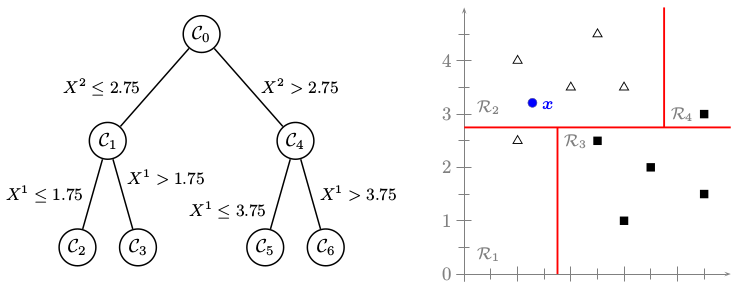
\includegraphics[scale=0.5]{img/decision_tree_simple_example}
    \caption{Decision tree of depth 2 for 10 elements belonging to 2 classes}
    \label{fig:decision_tree_simple_example}
\end{figure}


Naive bayesian

SVM (binary case) + kernel trick + multi-class (one-versus-one or one-versus-all)

The Support Vector Machine (SVM) is a method used for classification and regression. A support vector machine constructs a hyper-plane or set of hyper-planes in a high or infinite dimensional space, which can be used for classification, regression or other tasks. Intuitively, a good separation is achieved by the hyper-plane that has the largest distance to the nearest training data points of any class (so-called functional margin), since in general the larger the margin the lower the generalization error of the classifier.

To generalize SVM to the case of multi-class, multiple approaches are possible:
\begin{itemize}
    \item \enquote{one-versus-one}: train a separate classifier for each different pair of labels. This leads to $\frac{N (N - 1)}{2}$ classifiers
    \item \enquote{one-versus-all}: train a single classifier per class, with the samples of that class as positive samples and all other samples as negatives
\end{itemize}

Kernel trick:
to use the linear SVM for non-linear data: project the data in a new feature H space thanks to an application and then reserch for maximum margin hyperplan in H
to make sure that the new problem has a unique solution, 
must satisfy the Mercer's condition or simply it must be a positiv-definit matrix

\begin{itemize}
    \item \textbf{Linear} : $k(x, y) = \langle \vec{x} , \vec{y} \rangle + C = x^T y + C$
    \item \textbf{Polynomial}: $k(x, y) = (\gamma \cdot \langle \vec{x} , \vec{y} \rangle + C)^d = (\gamma \times x^T y + C)^d$
    \item \textbf{Radial Basis Function (RBF)}: $k(x, y) = \exp \left( - \gamma \lVert x - y \rVert ^2 \right)$
    \item \textbf{Chi-Square}: $\displaystyle k(x, y) = 1 - \sum_{i=1}^n \frac{(x_i-y_i)^2}{\frac{1}{2} (x_i+y_i)}$
    
    A modified version presented in \cite{Vedaldi2010} of this kernel is the \textbf{Additive Chi-Square} kernel :
    $\displaystyle k(x, y) = \sum_{i=1}^n \frac{2 (x_i - y_i)}{x_i + y_i} $
\end{itemize}

The adjustable parameters of these kernels are $d$, $\gamma$, $C$ and must be choosen according to the problem.

SGD classifier + loss function + regularization term% http://scikit-learn.org/stable/modules/sgd.html#mathematical-formulation

CNN

inspired by the neural system composed of different layers and communication shemes
recent years: use of the adjectiv "deep" to qualify NN: many layers

Different types of layers:
% http://cs231n.github.io/convolutional-networks/
% http://caffe.berkeleyvision.org/tutorial/layers.html
% Vision
- convolutional (give the name of the type of NN) : The Convolution layer convolves the input image with a set of learnable filters, each producing one feature map in the output image.
- max pooling
- normalization layer % http://stats.stackexchange.com/a/161200
% Loss layer
- sigmoid
% Activation / Neuron Layers
- ReLu